








\begin{figure*}[t]
     \centering
     \hspace*{\fill}\begin{subfigure}[b]{.44\linewidth}
         \centering
         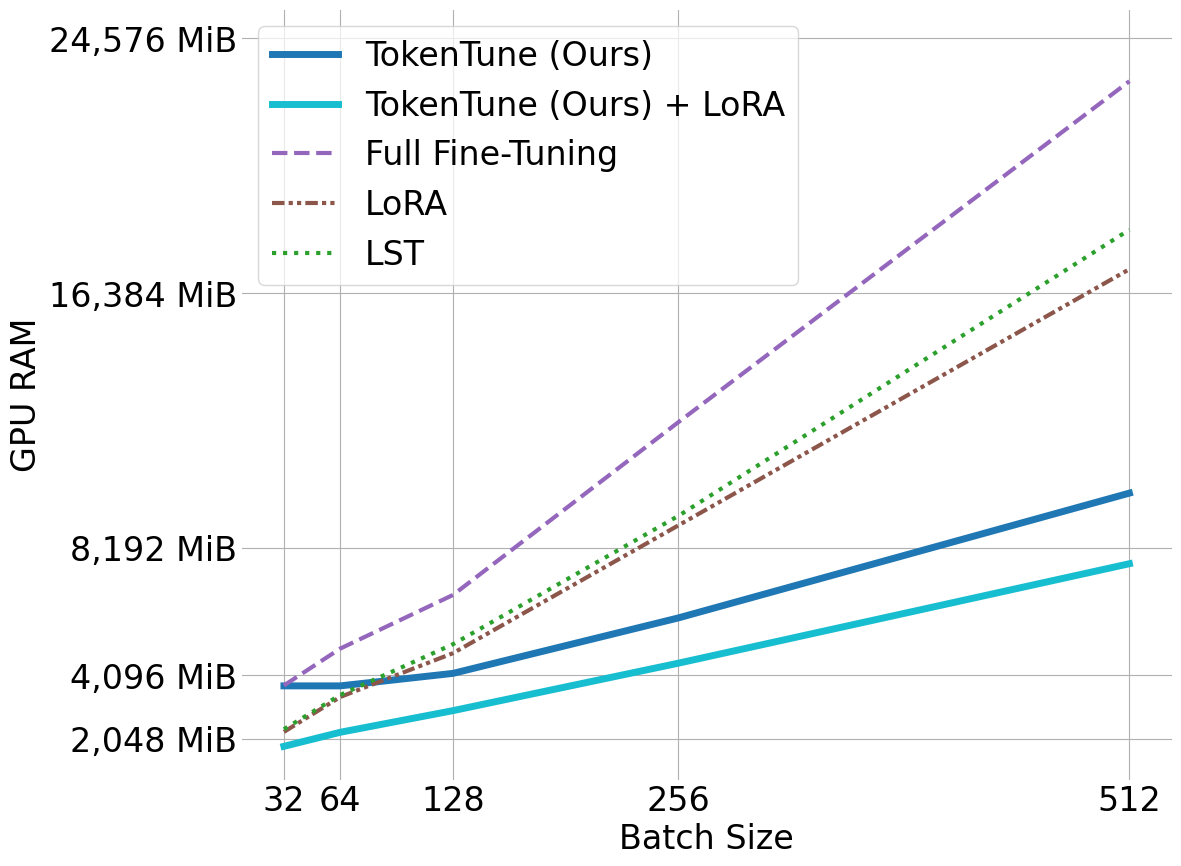
\includegraphics[width=\linewidth]{figures/bs_7.png}
\label{fig:ram}
     \end{subfigure}
     \hfill
     \begin{subfigure}[b]{.44\linewidth}
         \centering
         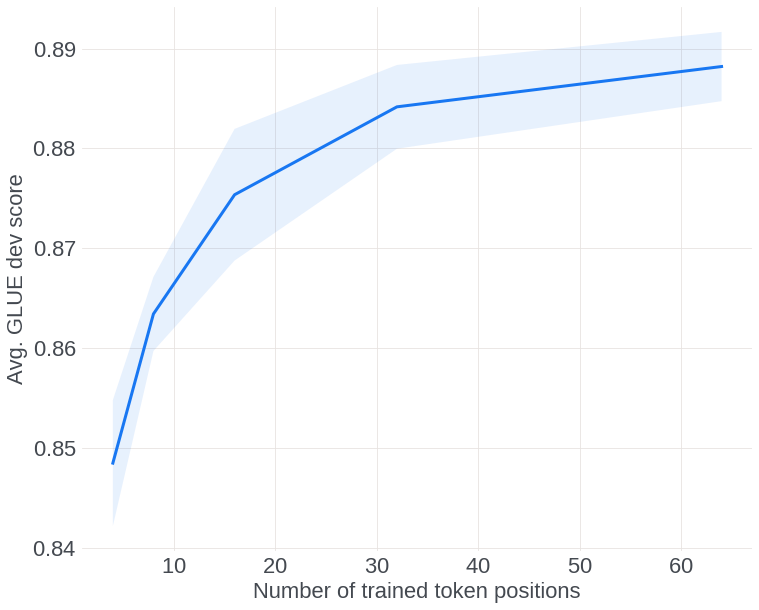
\includegraphics[width=\linewidth]{figures/pl_4.png}
\label{fig:prefix length}
     \end{subfigure}
     \hspace*{\fill}\caption{(left) We plot the GPU memory required to train \textsc{Bert}-base on the CoLA task given varying batch sizes. We compare our approach with two PEFT approaches: Ladder Side Tuning (LST) and LoRA. 
    (right) We plot the  mean and standard deviation performance on the dev set of five runs when training \textsc{Bert}-base on two tasks from the GLUE benchmark: MRPC and STS-B. We use our memory efficient fine-tuning approach with a different number of selected input tokens for the gradient computation.}
    \label{fig:graphs}
\end{figure*}

\section{Application to Medium-Size Encoders}  \label{sec:exp:medium}

Alternative methods such as zero-shot learning or prompting usually underperform fine-tuning \citep{DBLP:conf/nips/BrownMRSKDNSSAA20}. Thus, in many cases, fine-tuning medium size language models may offer a better balance in terms of cost and performance, compared with fine-tuning large language models (LLMs) or conditioning their outputs with prompt approaches \citep{DBLP:conf/iclr/LiTLH22, DBLP:conf/naacl/SchickS21}. Medium-size models may also be used as individual components, co-trained to encode information for a larger system \citep{pfeiffer_23}. Finally, as detailed in \Cref{sec:app:memorycomplexity:bkd}, the distribution of the GPU memory usage may be very different given the order of magnitude of the fine-tuned model's number of parameters. For large-size models, the majority of the memory is often dedicated to storing parameters and optimizer states, thus maximizing the relevance of PEFT approaches. For medium-size language models, fine-tuned with large batch sizes, the majority of the memory may be dedicated to storing the intermediate activation, thus maximizing the impact of \method.
























\subsection{Downstream Task Performance}



We first validate the relevance of our method on the GLUE benchmark \citep{wang_18}. 
We use a similar hyper-parameter search space as in \citep{zaken_22}, by performing a cross validation on the dev set using a learning rate in $[5e^{-5}, 3e^{-5}, 2e^{-5}, 1e^{-5}]$. We set the batch size to $16$ and perform $3$ epochs on large datasets and $20$ epochs on small ones (MRPC, STS-B, CoLA). We use \textsc{Bert}-large \citep{devlin_19} and either fine-tune the model fully, or use \method and propagate the gradient through $16$ input positions. We then evaluate our model on the test set and report the results in Table~\ref{table:glue}.

As shown in the second part of Table~\ref{table:glue}, the average GLUE score of \method is comparable to that of full fine-tuning, thus empirically validating the effectiveness of our approach.Table~\ref{table:glue} also shows that \method either outperforms or performs similarly to existing SOTA approaches.
Precisely speaking, the performance of these memory-efficient fine-tuning methods, including \method, is often slightly worse than that of full fine-tuning.
In comparison to full fine-tuning, some amount of performance loss with these methods is expected as 
they approximate or simplify the optimization process of full fine-tuning to reduce memory footprint.
We hypothesize that some tasks, such as QQP and QNLI, are more difficult, or sensitive to overfitting than others,
given that updating a small proportion of model parameters or using only a subset of input tokens for gradient computation 
achieves suboptimal performances on those tasks in most cases.
The former case would require the development of sophisticated techniques to more effectively select a subset of parameters or input tokens to optimize,
while the latter case may benefit from the use of regularization techniques for neural networks, including \citet{DBLP:conf/iclr/GoukHP21,DBLP:conf/iclr/ForetKMN21,DBLP:conf/nips/LiZ21},
the investigation of which we leave for future studies.



\subsection{Ratio of Tuned Input Positions} \label{sec:medium:ratio}

Given our token-selective fine-tuning approach, we then evaluate the impact of the number of frozen input positions on the performance. We use our selective procedure to fine-tune \textsc{Bert}-base on two tasks from the GLUE benchmark: MRPC and STS-B. 
We set the hyper-parameters as follows: $5e^{-5}$ for the learning rate, $32$ for the batch size and $4$ epochs.
We use different values for $k$ (i.e., the number of trained input positions), ranging between $4$ and $64$. We report in Figure~\ref{fig:graphs} (right), the average performance on the dev set of the tasks.\footnote{We provide some descriptive statistics in Appendix~\ref{app:stats_desc} to better understand how the absolute number of frozen input positions relates with the relative number of frozen input positions. The statistics include distribution of the sentence length for the two subtasks (MRPC and STS-B) used to produce Figure~\ref{fig:graphs} (right).}

As seen in Figure~\ref{fig:graphs}, the performance increases from $84.8$ to $88.8$ as the number of trained positions increases from $4$ to $64$. However, by only tuning $32$ positions, we already reach an average performance of $88.4$, close to the $88.8$ obtained by training $64$ input positions.
Our method surpasses the performance of freezing some bottom layers, as shown in \citep{lee_19}, where only tuning the four bottom layers resulted in a 10\% decrease in performance on the GLUE benchmark.






\begin{table*}[t]
    \centering
\caption{Few-shot evaluation on question-answering benchmarks including: AI2 Reasoning Challenge (25-shot) \citep{clark_18}, MMLU (5-shot) \citep{hendrycks_21}, HellaSwag (10-shot) \citep{zellers19}, TruthfulQA (0-shot) \citep{lin_22}, and WinoGrande (0-shot) \citep{DBLP:conf/aaai/SakaguchiBBC20}. We use the evaluation scripts and prompt formatting from the "Language Model Evaluation Harness" \citep{eval-harness}. We report the average accuracy on five MMLU ethics tasks and WinoGrande, the normed accuracy on ARC and HellaSwag, and the MC2 score on TruthfulQA. 
   	We indicate in \textbf{bold} the best result for each task.
   	We report the results with the raw Llama2-7B model \citep{touvron_23} and the Llama2-7B fine-tuned on the Platypus curated instruction dataset \citep{lee_23} using LoRA \citep{hu_22}, QLoRA \citep{dettmers_23} and the proposed \method. When fine-tuning with \method, we select 30\% of the tokens for the gradient computation.}
    \label{tab:llm-perf}

	\setlength{\tabcolsep}{1pt}    


  


\resizebox{.98\textwidth}{!}{

\begin{tabularx}{\textwidth}{lYYYYYY}
	\toprule
	\makecell[c]{{Method}} & {MMLU} & {ARC} & \makecell[c]{{Hella}\\{Swag}} & \makecell[c]{{Truthful}\\{QA}} & \makecell[c]{{Wino}\\{Grande}} & {Avg. $\uparrow$}\\
	\midrule
	Llama 7B & 64.44 & 52.39 & \textbf{78.97} & 38.97 & 68.90 & 60.73\\\midrule
	Llama 7B w/ LoRA & \textbf{65.89} & 55.38 & 78.76 & 42.64 & 68.35 & 62.20\\
	\rowcolor{lightcyan}
	Llama 7B w/ LoRA+\method (Ours) & 65.42 & 54.01 & 78.82 & \textbf{43.78} & 68.35 & 62.08\\\midrule
	Llama 7B w/ QLoRA & 65.08 & \textbf{56.06} & 78.60 & 43.64 & 69.38 & \textbf{62.55}\\
	\rowcolor{lightcyan}
	Llama 7B w/ QLoRA+\method (Ours) & 65.78 & 53.92 & 78.74 & 41.91 & 69.38 & 61.95\\\midrule
	\rowcolor{lightcyan}
	Llama 7B w/ \method (Ours) & 63.06 & 53.07 & 77.90 & 42.18 & \textbf{69.93} & 61.23\\
	\bottomrule
\end{tabularx}

} 

\end{table*}

\subsection{GPU Memory Impact} \label{sec:medium:mem}

Finally, we analyze the GPU memory required to fine-tune models using various approaches.  We train our \textsc{Bert}-base model for $100$ steps on the CoLA task using various batch sizes and report the peak GPU memory used. We compare with two other PEFT fine-tuning approaches close to ours: Ladder Side Tuning \citep{sung2022lst} and LoRA \citep{hu_22}. LoRA freezes most of the model parameters, while only training additional low-rank matrices, whose weights are added to the backbone network. Ladder Side Tuning (LST) freezes the model parameters but trains a side-network with smaller dimensions, taking as input intermediate activations from the backbone model.

\Cref{fig:graphs} shows the evolution of the required GPU memory with respect to the batch size. GPU memory increases with the batch size for every approach. \method is more memory efficient by a large margin. When using a batch size of $512$, it requires two times less memory than full fine-tuning: $23,196$ MiB needed for full fine-tuning is reduced to $9,952$ MiB with our method.

All methods minimize GPU memory usage. LoRA and LST reduce the memory required to store optimizer states and parameter gradients, while our method reduces  the memory for storing intermediate activations. 
Interestingly enough, it is possible to use these approaches in conjunction to reduce the memory for all three contributions. 
Fig.~\ref{fig:graphs} shows that we can further reduce the memory by combining \method with LoRA, thus requiring only $7,682$ MiB with a batch size of 512, a third of the memory used for full fine-tuning.

















